
\begin{figure}[H]
    \centering
    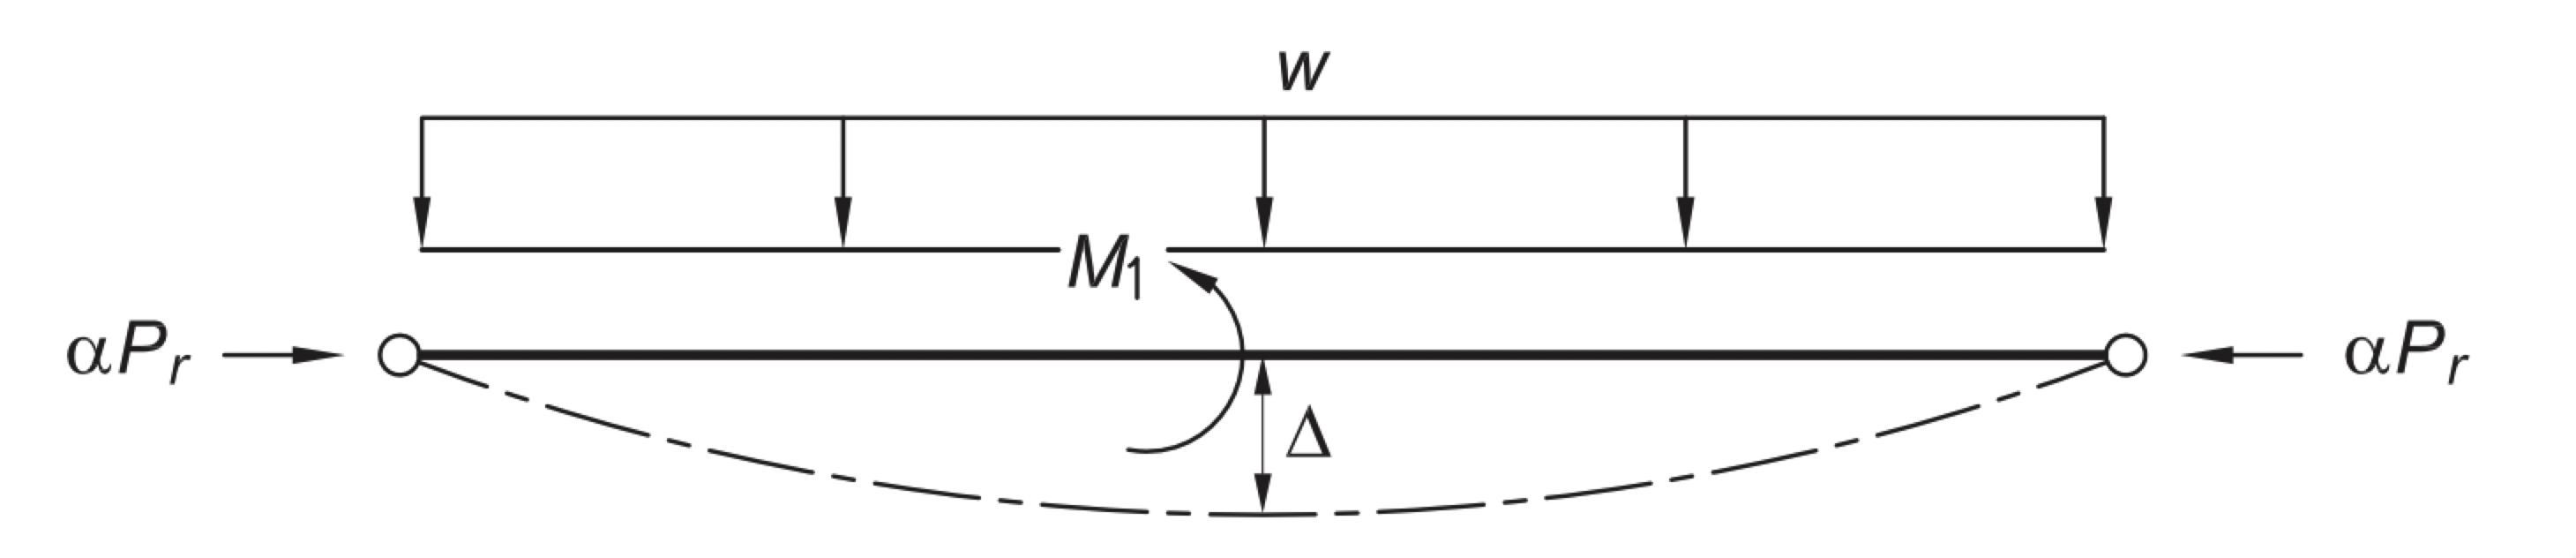
\includegraphics[width=0.6\linewidth]{Examples/frame-1003/img/frame-1003.png}
    \caption{Simply supported span with a uniformly distributed load \(w(x) \FrameBasis_z\).}
    \label{fig:1003-conf}
\end{figure}

This problem addresses a common oversight in the implementation of 
distributed loading under a corotational transformation. 
Distributed loads are most commonly used to model gravitational loads on members. 
In order to model such an effect under corotational kinematics, the loads must be applied in the inertial basis, otherwise they will act as follower loads that rotate with the corotational basis.  

This phenomenon is illustrated by a simply supported span subjected to a uniformly distributed conservative force. 
A similar problem was considered by \cite{desouza2000forcebased}.


\Cref{fig:1003-soln} shows load-displacement curves for the cases under consideration. 

\begin{figure}[H]
\centering
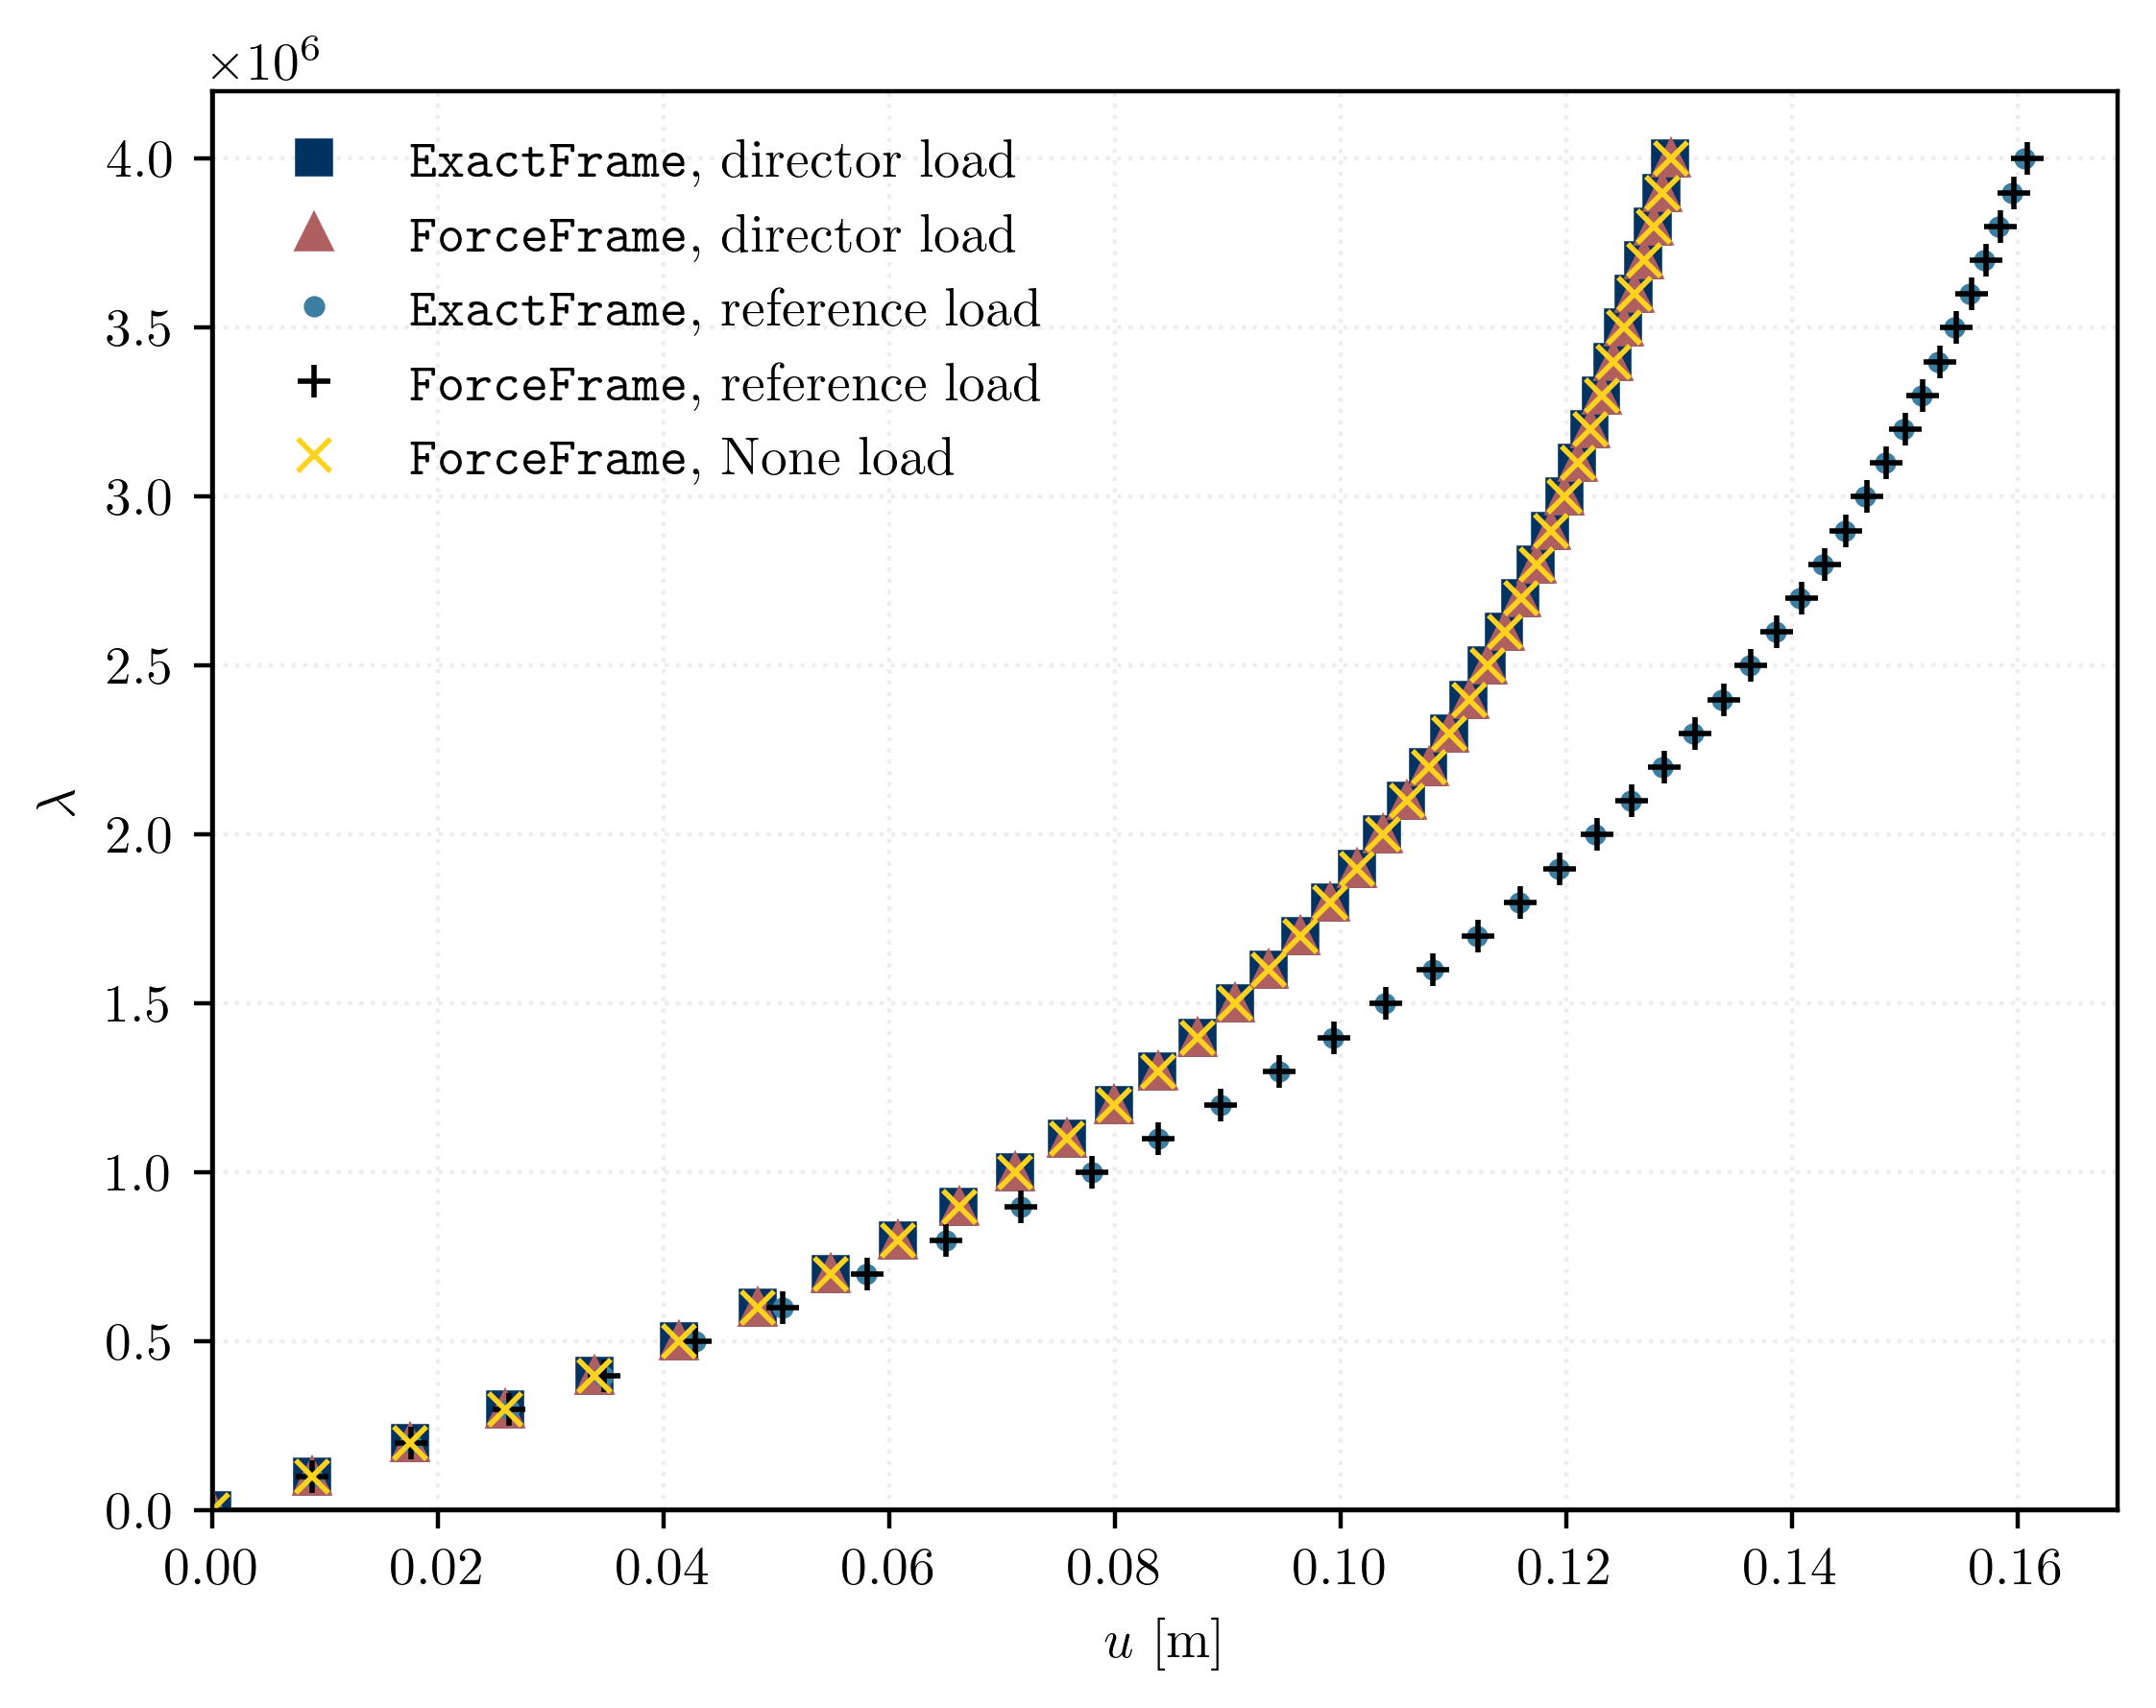
\includegraphics[width=0.75\linewidth]{Examples/frame-1003/img/1003-bases.png}
\caption{Simulated displacements for Example~\ref{sec:frame-1003}.}
\label{fig:1003-soln}
\end{figure}

